\subsection{\large{Сервис запуска математических методов}}
\addcontentsline{toc}{subsection}{\large{Сервис запуска математических методов}}

Детальная архитектура сервиса запуска математических методов представлена на диаграмме компонент
(см. рис\ \ref{pic:architecture__executor-component}).

\begin{figure}[H]
	\hspace*{-2.5 cm}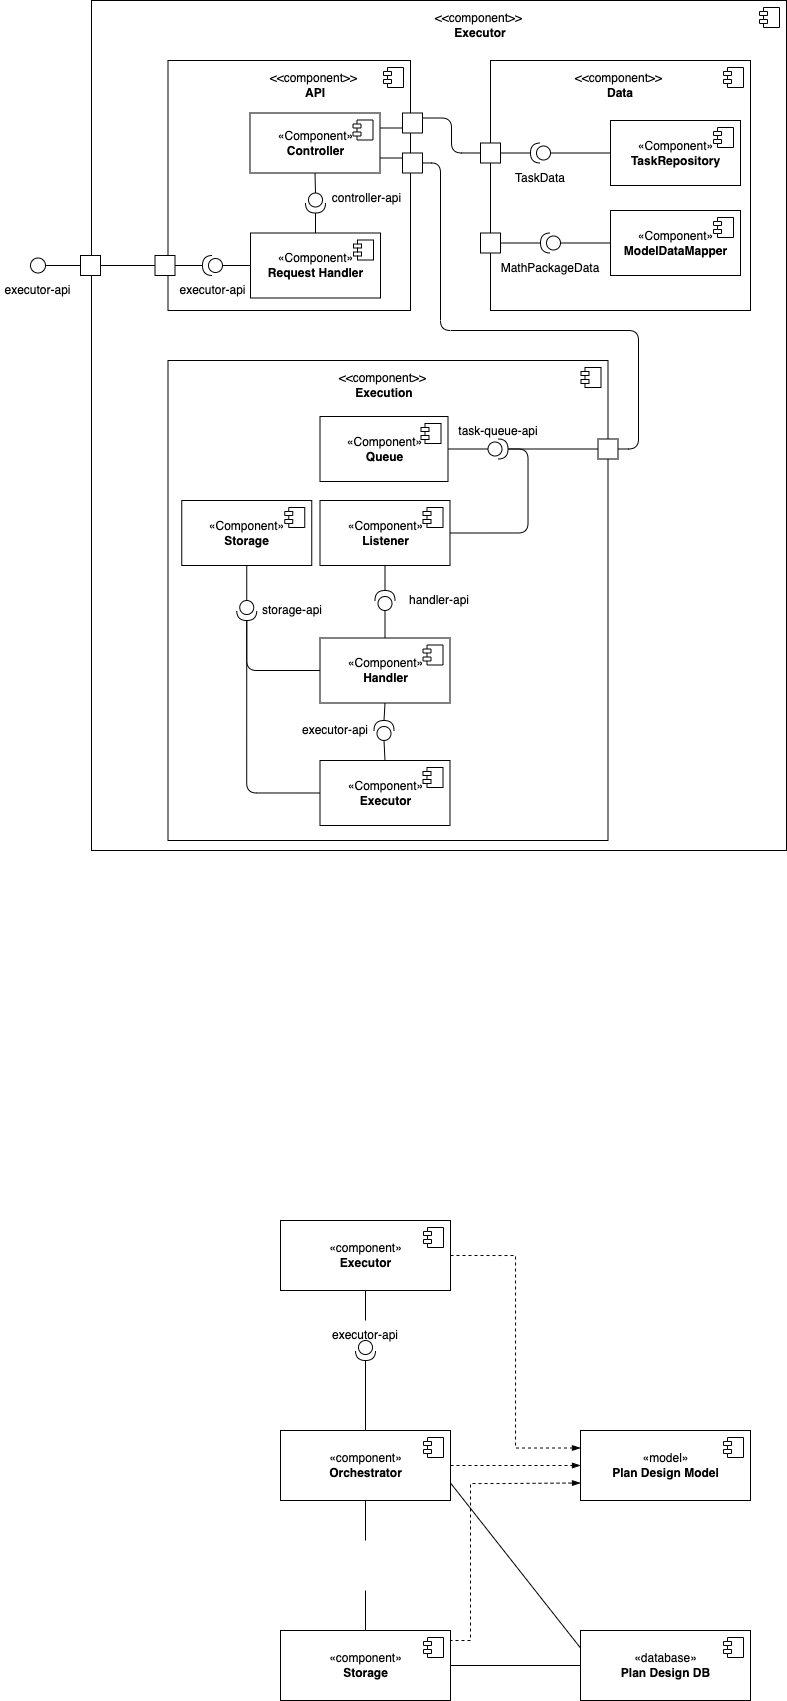
\includegraphics[width=\textwidth]{architecture/pictures/executor/component}
	\caption{Диаграмма компонент сервиса запуска математических методов}
	\label{pic:architecture__executor-component}
\end{figure}
\vskip 5 mm

Сервис представлен следующими компонентами:
\begin{enumerate}
	\item {
		\textbf{API} -- отвечает за предоставление REST API и отправки задачи в очередь.
		\begin{itemize}
			\item \textit{Request Handler}
			\item \textit{Controller}
		\end{itemize}
	}
	\item {
		\textbf{Data} -- отвечает за получение и сохранение данных.
		\begin{itemize}
			\item \textit{TaskRepository}
			\item \textit{ModelDataMapper}
		\end{itemize}
	}
	\item {
		\textbf{Execution} -- отвечает за запуск метода в отдельном процессе.
		\begin{itemize}
			\item \textit{Queue}
			\item \textit{Listener}
			\item \textit{Storage}
			\item \textit{Handler}
			\item \textit{Executor}
		\end{itemize}
	}
\end{enumerate}